\chapter{Background}
Others have approached the objectives highlighted in \autoref{chap:Intro} in the form of Trail Running Applications, and Recommender systems. Therefore, researching related works and existing solutions is imperative to understanding these topic areas and help advise the approach taken by the project.

\section{Trail Running Applications} \label{sec:TrailRunningApplications}
Many applications provide the functionality to support trail running. They equip the user with an interface that empowers them with tools to create and discover trails via web applications and\\or mobile applications such as Strava. 

\subsubsection{Strava}
Strava is a popular application that provides trail running services to its users with its website and mobile application \cite{strava}.  The primary focus is fitness and competition.  It does this by allowing users to upload \acrfull{gps} data and recorded times of runs they have performed on a trail. These details are used to populate leader-boards and generate rankings on trails.


There are other many other trail running applications such as \acrfull{os} Maps, Mapometer and others. They all provide a Map Interface that allows users to create trails by clicking on points on the map and connecting the points with a line. They include searches, maps, and details on trails to help their users find what type of trail they wish to use. However, they all fail at giving personalised trails to each user. Although they use location information (trails in the user's immediate area), they do not use any information retrieval techniques to get tailored trails to each user, also known as Recommender Systems explained in section \ref{sec:RecSystems}

\begin{figure}[ht]
    \centering
    \includegraphics[width=\textwidth]{images/os-maps-editor.png}
    \caption{OS Maps trail editor that allows user to create trails by clicking on points on the map}
    \label{fig:osMapsEditor}
\end{figure}

\section{Recommender Systems} \label{sec:RecSystems}
Recommender systems are a type of Information Filtering System that provide suggestions personalised to an intended user \cite{ricci2011introduction}.  Recommender systems arose as a solution to the problem of too many options, especially with the age of the Internet where businesses can make available even more products and/or services \cite{rishabh2019recommender}.  By trying to determine each users preferences, the system can suggest items that are appropriate to each specific user.  The term ``item" can refer to almost any product or service that requires a users choice, for trail running, it refers to the trails. We can see  Recommender Systems in most areas such as,  movies,  products, news, people and so on.

\subsection{Why Recommender Systems} \label{subsec:WhyRecSystems}
In 1896, the Italian Economist Vilfredo Pareto proposed a theory that for events, \textit{``80\% of the effects, come from 20\% of the causes" \cite{sanders1987pareto}}. This theory is known as the Pareto Principle and is more commonly know as the 80/20 rule. Traditionally, this rule is a popular maxim in business and strategy management, based on the idea that 80\% of sales can be generated by 20\% of the items being offered, commonly referred to as the ``best selling items".

However, in a 2004 article in \textbf{Wired} Magazine, Chris Anderson observed that on the internet, businesses can be more profitable by offering a larger number of niche, hard-to-find products \cite{brynjolfsson2011goodbye}. This phenomenon was coined \textbf{the Long Tail Effect}, further discussed in Chris Anderson's book \textit{``The Long Tail: Why the Future of Business Is Selling Less of More"} \cite{anderson2006long}. He explains that this new trend is is due to the the improvement in technology that enables users to search and discover more easily. 

\begin{figure}[htb!]
    \centering
    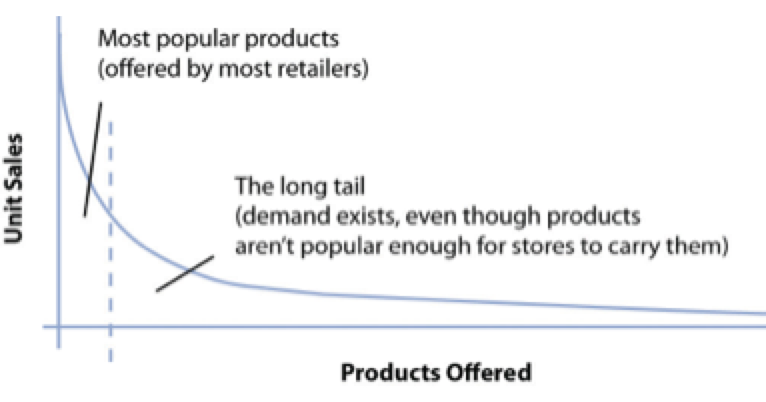
\includegraphics[width=0.75\textwidth]{long-tail.png}
    \caption{The long tail effect \cite{longtaileffect}}
    \label{fig:longtail}
\end{figure}

It especially was strengthened by the advent of Recommender Systems. By offering more personalised items to users, we can expose users to these hard-to-find items that would have been apparent in on a popularity list. Proof of the advantages Recommender Systems offer can be seen by the major companies that take advantage of these systems.


\subsubsection{Amazon} 
Amazon is a behemoth multi-billion dollar online retail company. According to Statista, in 2018, they generated 232.89 billion dollars \cite{statista}. In a 2013 article by Mckinsey \& Company, it is reported that 35\% of Amazon's revenue comes from its recommendation System. 

\subsubsection{Netflix}
Netflix is an online video streaming platform that offers thousands of TV Series and Movies to it's millions of users. Netflix uses a Recommender System not only to personalise the videos offered to the user, but also the artwork that is used as the thumbnail\footnote{a cover image for a video} for the video \cite{josefina2018netflix}.

These are just a few examples of platforms that benefit from Recommender systems \cite{polatidis2013recommender}.

\subsection{Machine Learning Approach} \label{subsec:mlApproach}
Machine Learning is a study of Artificial Intelligence that uses algorithms and models to enable computer systems learn how to perform tasks using data without the need for explicit instructions to be given \cite{michie1994machine}. Machine learning models are used for a variety of tasks such as classification\footnote{differentiation between items}, facial recognition, regression analysis and so on.

Regression Analysis is a set of techniques that discover relationships between variables in data \cite{chatterjee2015regression}. By trying to find a best fit between variables in data, you can discover the relationship between them and also predict values for new variables. Regression analysis can also be described as a predictive analysis, hence, Recommender Systems can be classified as a Regression Analysis problem, as the system try's to predict a user's predicted rating of an Item. Hence we have a means to creating a Recommender System using Machine learning Methods.

\section{GraphQL over REST}
Web applications consists of two main parts: the client, which contains the user interface the user interacts with, and the server, which provides the resources needed to be consumed by the client. In recent years, \acrfull{rest} has quickly been adopted in industry as the standard for creating a server \acrfull{api} \cite{guy2015rest}. They allow the client to access the resources provided in the server via stateless operations with the use of a \acrfull{url}. However one of the main problems with \acrshort{rest} is it's lack of flexibility. The resources in \acrshort{rest} are exposed via endpoints. The shape of the data returned to the client by theses endpoints are defined by the server. This can lead to problems of \gls{over-fetching} and \gls{under-fetching}. In \autoref{fig:restProblem}, we can see a standard \acrshort{rest} \acrshort{api} that exposes a users details, posts and followers via separate endpoints. The client is forced to make multiple requests to get the data required as each endpoint returns under-fetched. If the client requests only a users name from the user details endpoint, this leads to over-fetching of data.

\begin{figure}[htb!]
    \centering
    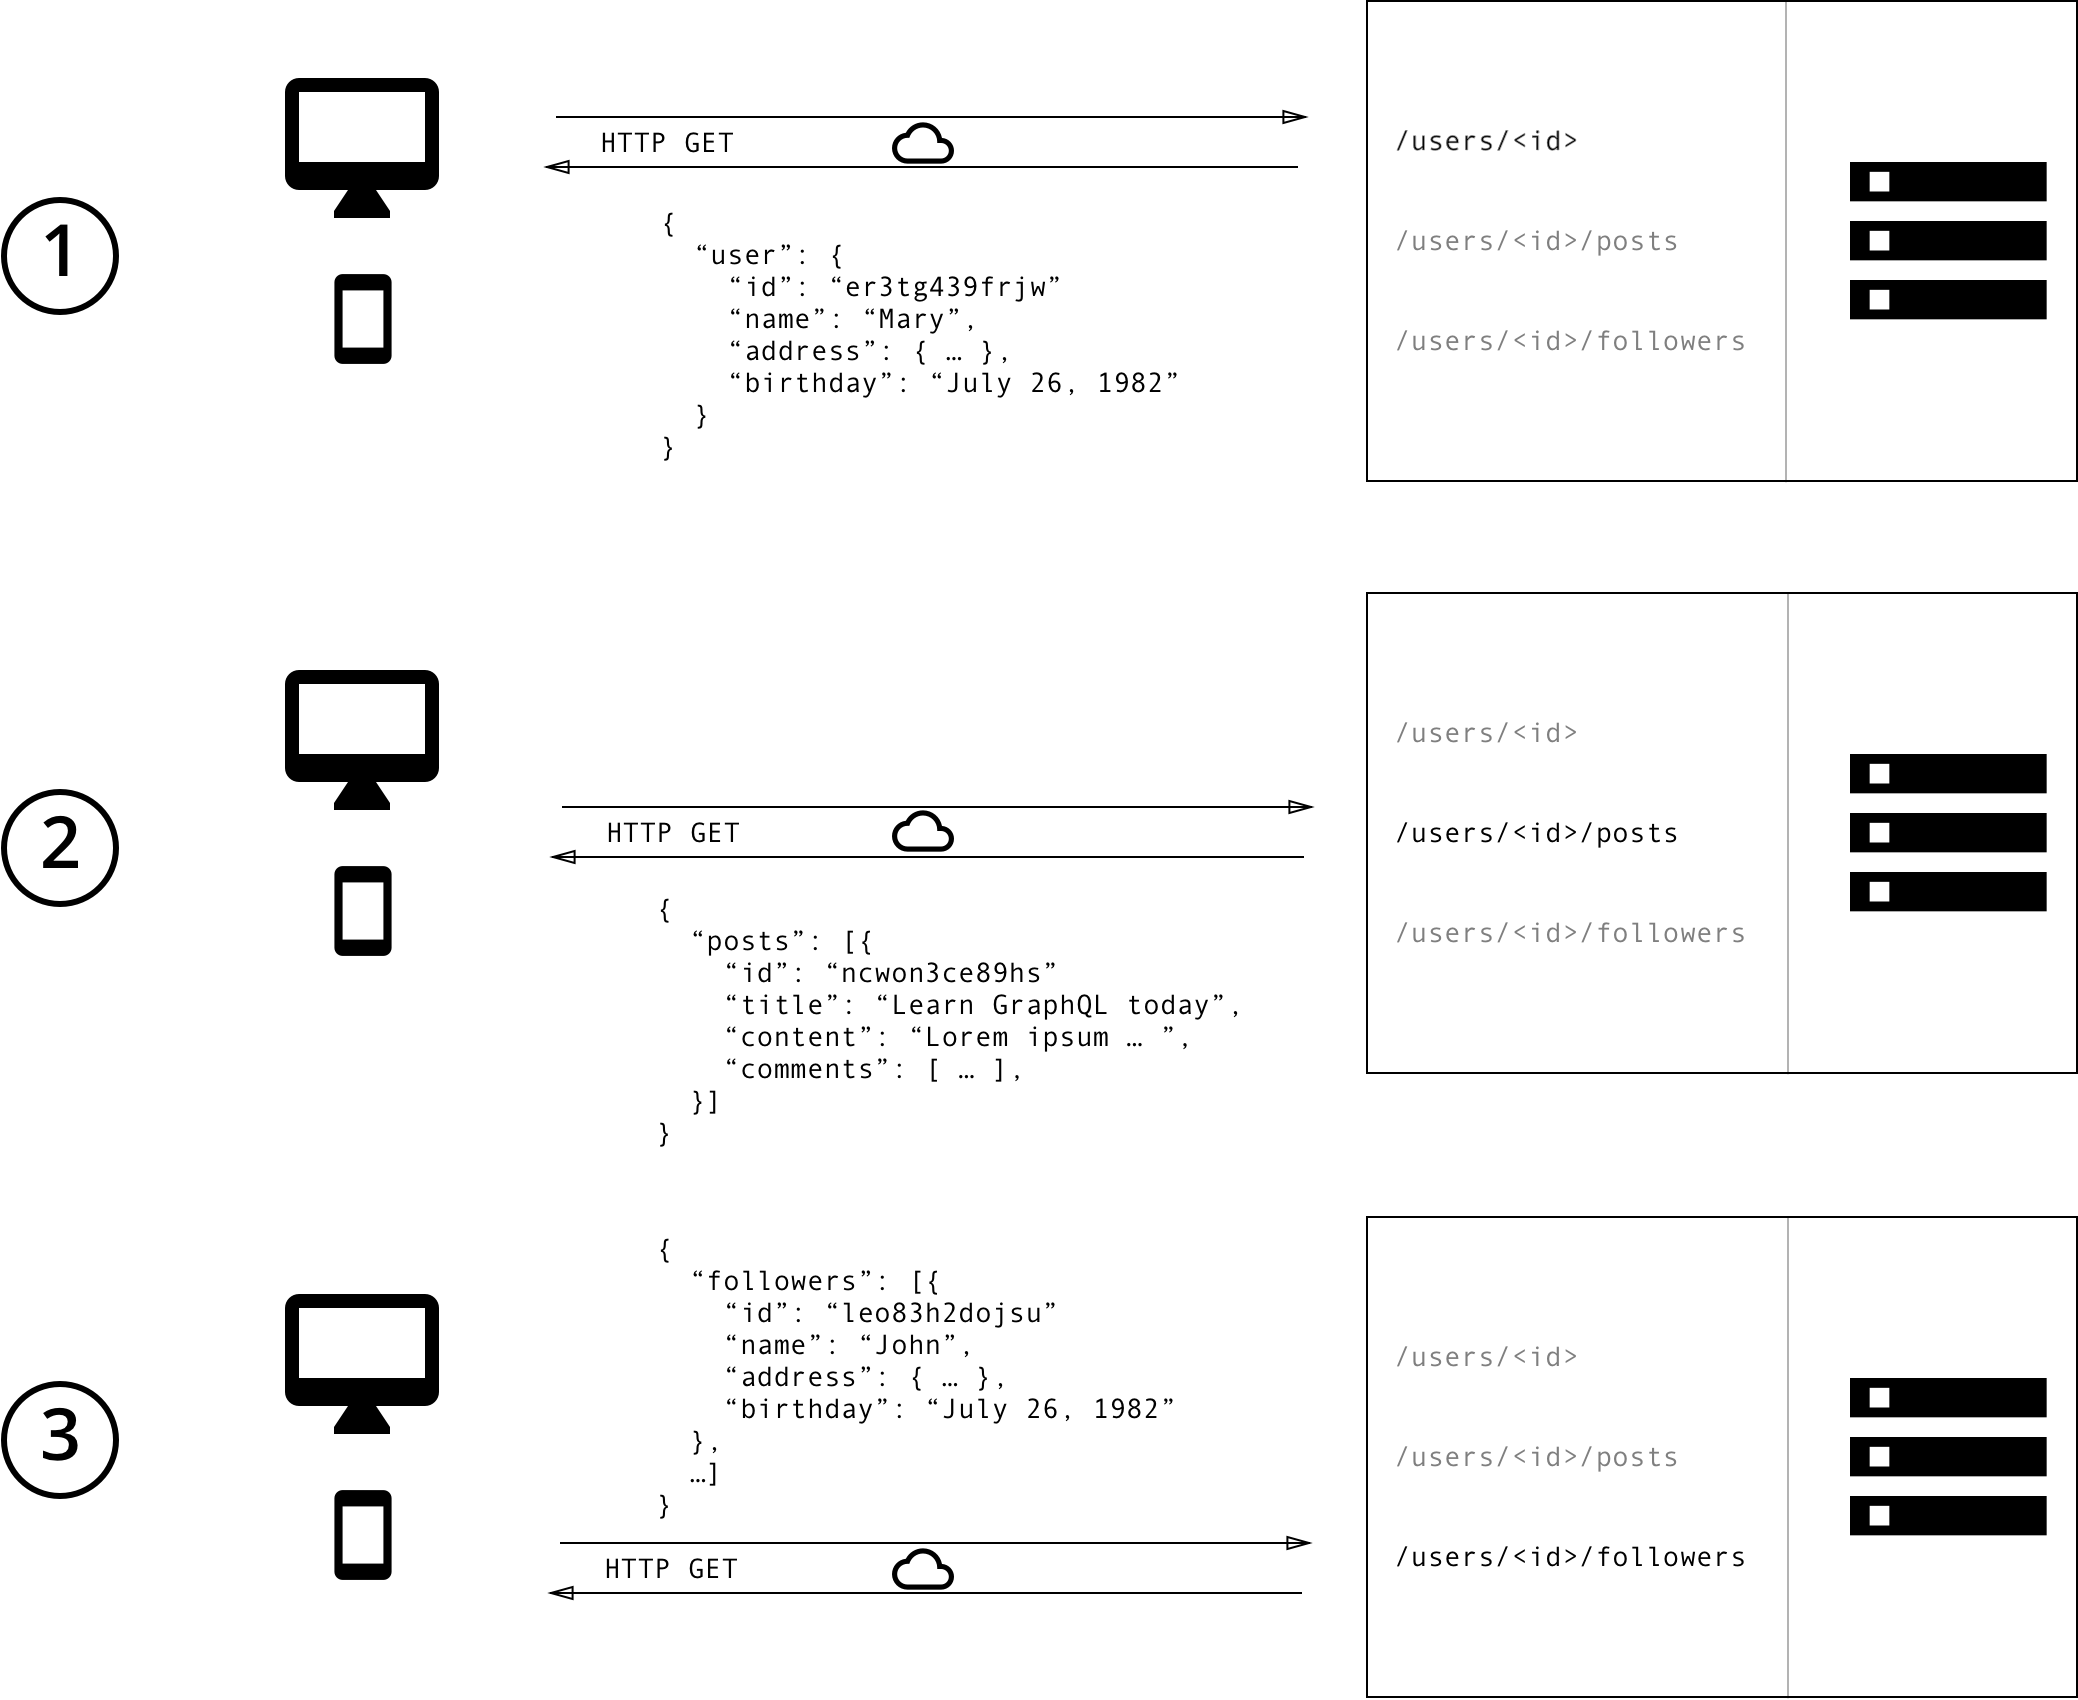
\includegraphics[width=0.75\textwidth]{problems-with-rest.png}
    \caption{REST having to make three separate requests to to three different endpoints to get the required data \cite{graphqlvsRest}}
    \label{fig:restProblem}
\end{figure}

GraphQL was introduced as a solution to the shortcomings with \acrshort{rest} GraphQL, created by Facebook in 2012, and then open sourced in 2015, is a query language for an \acrfull{api} and a run-time for fulfilling those queries with your existing data \cite{graphQl}.  Like \acrshort{rest}, GraphQL is used to expose resources to the client. However, GraphQl only exposes a single endpoint and the client defines the structure of the data that is required \cite{howToGraphQl}, eliminating the problem of over-fetching and over fetching. \autoref{fig:graphqlFix} shows how a GraphQL server can get the same data as the before, using only one request.

\begin{figure}[htb!]
    \centering
    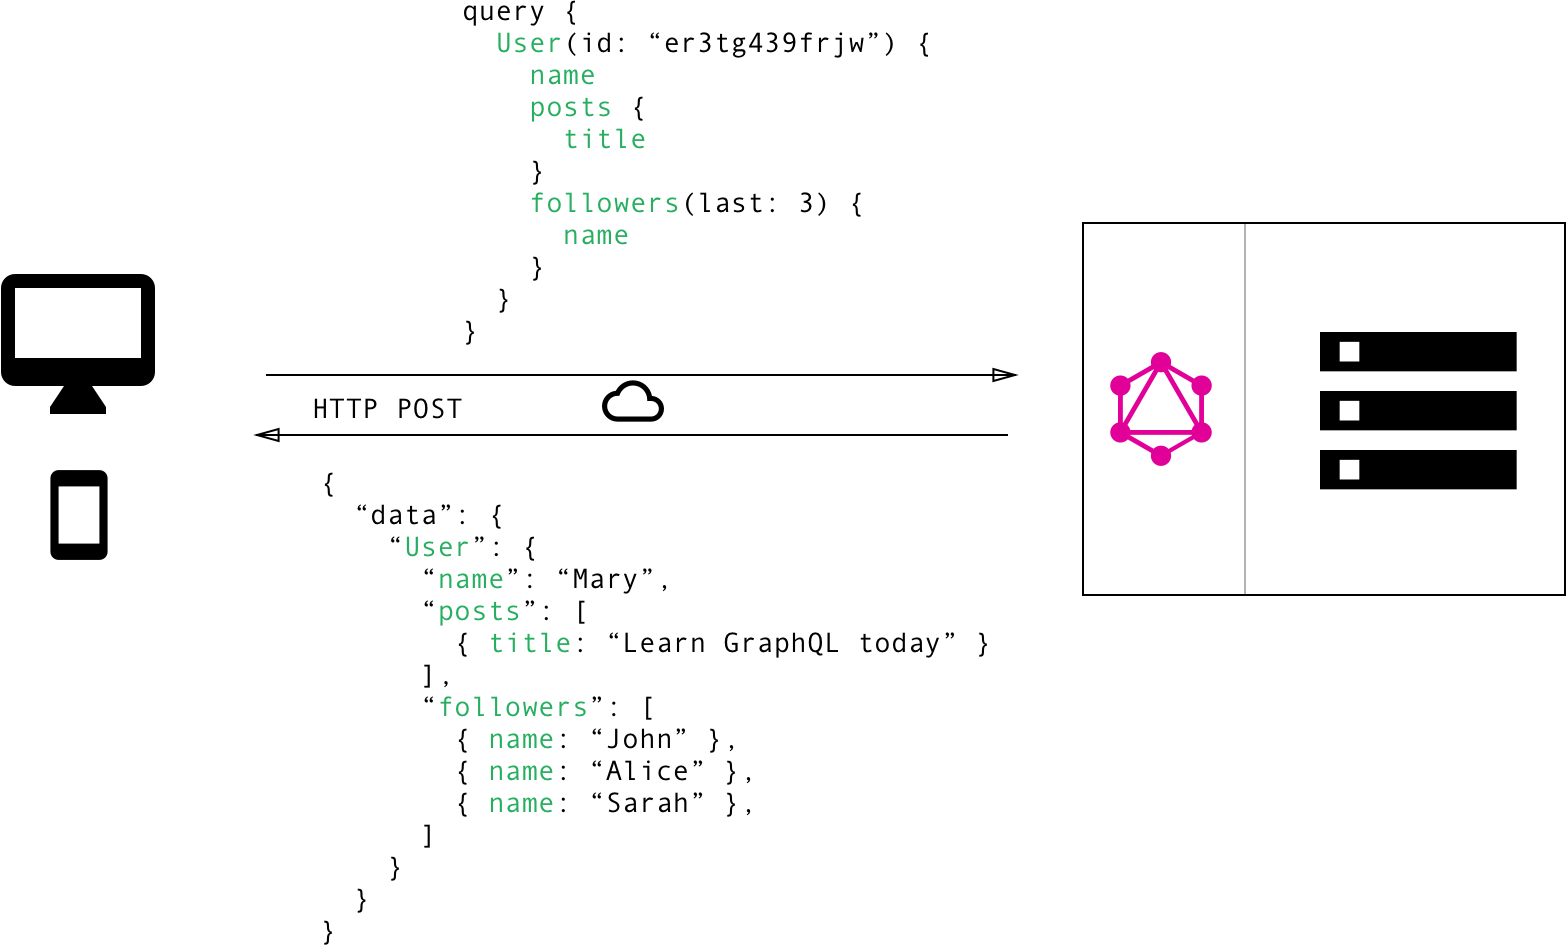
\includegraphics[width=0.75\textwidth]{fetching-graphql.png}
    \caption{GraphQl can perform retrieve the same required data using one request to one endpoint \cite{graphqlSolution}}
    \label{fig:graphqlFix}
\end{figure}

This is important in our application as in some scenarios where information is being retrieved, we would want to prevent over-fetching. To store trail information, a large number of coordinates per each trail needs to be stored. When a user is searching for a trail initially, only details such as the name of the trail, average rating and so on are required. Requesting all the coordinates would add unnecessary overhead to the system during communication between the client and server.